\section{Hardware Platform}
The platform used for the experiments is TI Hercules TMS5703137.\\
The platform is designed to conform to functional safety standards including ISO26262.
The platform employs a dual core lockstep processing using cortex R4. 
Some of the features which are important for providing AUTOSAR support are mentioned below.

\subsection{Architecture: Cortex-R4}
Cortex R4 processor is a midrange processor used in real-time systems.
It implements ARM-V7R Architecture and supports THUMB-2 technology for optimum code density and processing throughput.
The pipeline has single Arithmetic Logic Unit but uses limited dual-issuing to of instructions for efficient utilization of other resources such as registers.
The processor has Tightly coupled Memory(TCM) port for low latency and deterministic access to local RAM in addition to caches for high performance general memory.
The Level 1 memory and processor ports of Cortex R4 uses Error Correction Code(ECC) for greater reliability and address safety.
An overall component level diagram of Cortex-R4 is shown below:
\begin{figure}[h]
	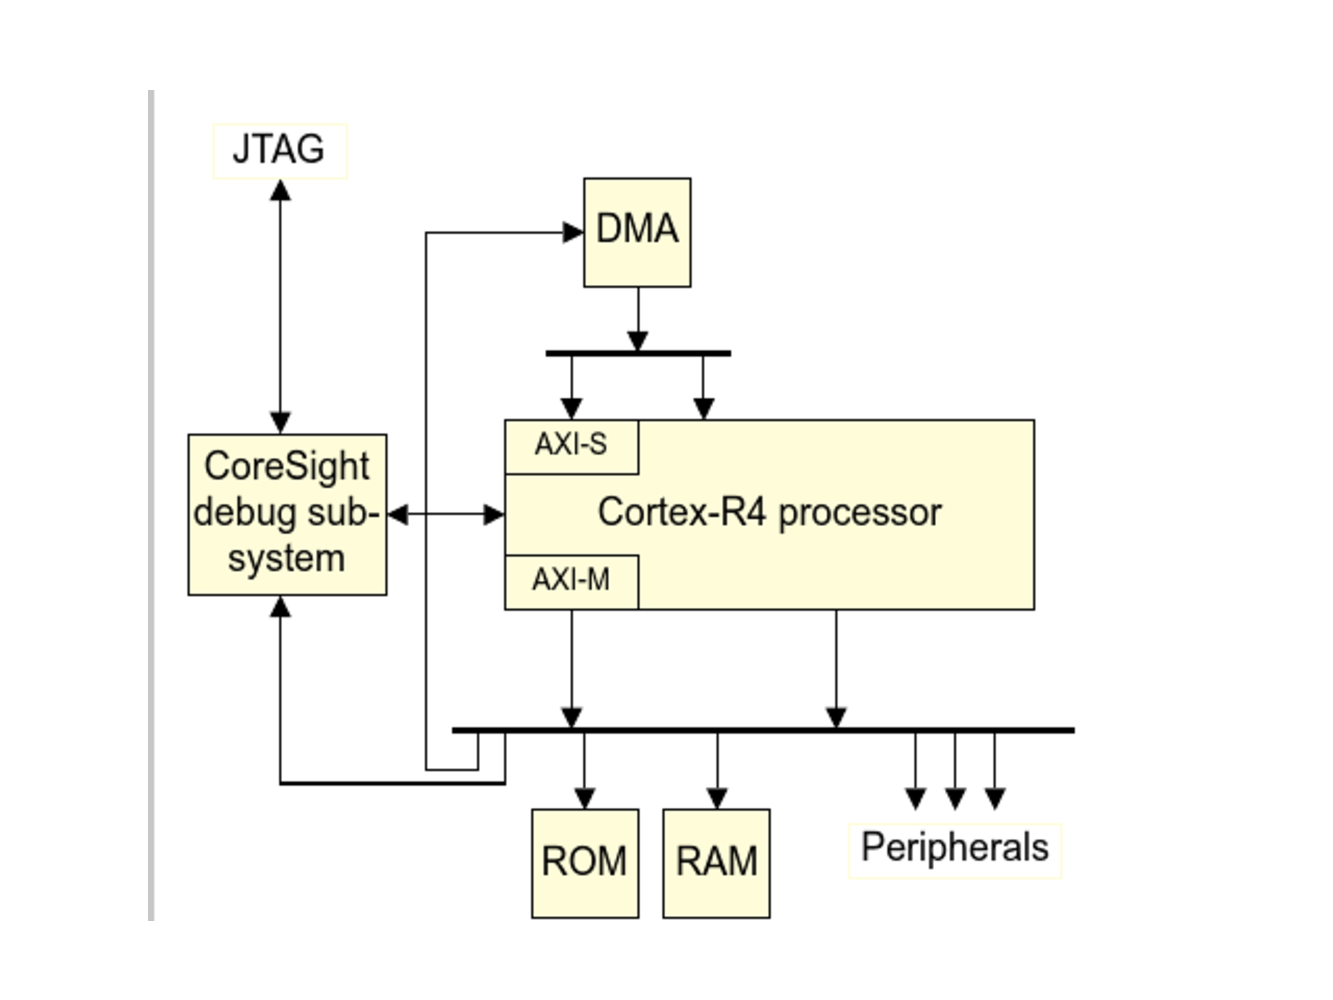
\includegraphics[scale = 0.5]{CortexR4}
\end{figure}

The main features of the Cortex-R4 are listed below:
\begin{itemize}
 \item A Dual issue integer unit with integral coresight logic.
 \item High speed Advanced Microprocessor Bus Architecture(AMBA) and Advance eXtensible Interface(AXI) for master and slave interfaces.
 \item Dynamic branch prediction with history buffer and 4-entry return stack.
 \item Low interrupt latency.
 \item Non Maskable Interrupt.
 \item Optional Floating point unit.
 \item Harvard L1 Memory system with:
 \begin{itemize}{}{}
 	\item Optional Tightly Coupled Memory(TCM) with support for error correction or parity checking.
 	\item Optional caches with error correction codes(ECC).
 	\item Optional ARM-V7R Memory Protection Unit(MPU).
 	\item Optional parity and error correction support for all RAM blocks.
 \end{itemize}
 \item An L2 Memory Interface with single 64-bit master AXI interface and 64 bit slave AXI interface to TCM RAM blocks and cache RAM blocks.
 \item A Performance measuring Unit(PMU).
 \item Vectored Interrupt Controller(VIC).
\end{itemize}

\subsection{Components}

\subsubsection{\textbf{TCM Interfaces}}

TCM Interface for Cortex-R4 are composed of two interfaces, ATCM and BTCM.
An ATCM usually holds the exception handler code that must be accessed at high speed without any cache miss.
BTCM meanwhile holds block of data for intensive operations such as Audio and Video processing.


\subsubsection{\textbf{Power Management}}

Processor includes number of processor features for power management:
\begin{itemize}
	\item Accurate branch and return prediction.
	\item Cache uses sequential access information to reduce the number of accesses.
	\item Extensive use of clocks and gates to disable the inputs to unused functional block.
\end{itemize}

\begin{flushleft}
Cortex-R4 supports 4 different power levels:
\end{flushleft}
\begin{itemize}
	\item \textbf{Run Mode}: The normal mode where all the functionalities of the processor are available.
	\item \textbf{Dormant Mode}:Dormant mode disables with processing logic but not the TCM and cache RAMs. Before entering the mode the processor state is saved to the memory and restored when exiting the mode.
	\item \textbf{Standby Mode}: In standby mode most of the clocks of the device will be disabled, while the device will be kept powered on.
	\item \textbf{Shutdown Mode}: In this mode entire device including cache and TCM logic are disable and should be saved to the external memory.
\end{itemize}

\subsubsection{\textbf{System Reset Levels}}
The processor has following reset inputs: nRESET, PRESETDBGn, nSYSPORESET, nCPUHALT.
Using the combination of given resets following reset modes can be realized: 
\begin{itemize}
	\item \textbf{Power On Reset}:Also known as hard reset or cold reset. Both nRESET and nSYSPORESET are asserted and this is done during initial system reset. This will reset entire system.
	\item \textbf{Processor Reset}:
	Also known as soft reset or warm-reset. nRESET is asserted while nSYSPORESET is set to 1.
	\item \textbf{Halt}: Both nSYSPORESET and nRESET are set to 1 , while nCPUHALT is asserted by setting to 0.
	\item \textbf{Normal Mode}: All three nRESET, nSYSPORESET and nCPUHALT are set to 1. One use case is doing DMA into TCM using the processor.
\end{itemize}

\subsection{Initialization}
Most of the architectural registers in the processor, such as r0-r14, s0-s31 and d0-15 are not reset. Thus these needs to be reset explicitly during the initialization phase.
So of the main activities to be carried out includes: programming registers like stack pointers, processor features and interface initialization and are mentioned below:
\subsubsection{MPU}
If the processor is built with Memory Protection Unit(MPU), before using it program and enable on of its region and enable MPU in system control registers.
If MPU regions are enabled, program them to enable access to TCM regions before using them.
\subsubsection{FPU}
If the processor is build with Floating Point Unit, enable it before accessing VFP instructions. This is done by enabling access to FPU in Coprocessor Access Registers.
Also enable FPU by setting the EN bit in FPEXC(Floating point Exception) register.
\subsubsection{Cache}
If the processor are build with instruction or data cache they must be invalidated before use otherwise the behavior is unpredictable.
If ECC is to be supported for the cache, it must be enabled before invalidating the cache by programming the Auxiliary Control Register. This enabled correct error code or parity bits are calculated.

\subsubsection{TCM}
TCM is not explicitly initialized by Processor and as such should be initialized as per the requirement.
Additionally main instruction may require data to be preloaded into TCM. There are multiple ways TCM memory can be preloaded and are listed below:
\begin{itemize}
	\item The boot code can copy the required data from ROM using the memory routine. For this TCM need to be enabled and separate base address to TCM during copy and normal program execution are provided.
	\item Boot code includes routine to copy data from the Debug Communications Channel(DCC) to TCM.
	\item Processor is put into debug halt state and Instruction Transfer Register(DBITR) is used to transfer data that is executed by the processor and overrides the boot code.
	\item SoC includes DMA device which can directly write the data from ROM code to TCM through AXI slave.
	\item Debug Access Port(DAP) can be used to generate AMBA transactions to write data directly to TCM through AXI slave.
\end{itemize}
Refer to Auxiliary Control Registers to check for initializing TCM with ECC\footnote{Error Correction Code}.
Processor can be pin configured to enable TCM at reset.
\section{CORTEX M0+}
A low area low power 2 stage pipelined architecture for low power modules.\\
compact with total of 56 instructions.\\
Uses AHB lite bus for communication with peripherals and uses 32 bit addressing for a total of upto 4gb of addressable memory.\\
Support two main control modes: Kernel mode and User mode.
User mode can be further divided in to two sub categories of privileged and non-privileged.\\
PSR or Programme status register has 3 main types: Application Program SR, Interrupt Program SR, Exception Program SR.\\
CMSIS Support package provided, which is a a standardized way to access peripheral registers and exception vectors.\\
Memory types can be: Normal, Device, Sharable, Strongly Ordered, Execute Never.\\

Order of execution of the program instructions can be guaranteed by:
\begin{itemize}
	\item Data Memory Barrier(DMB): Assures that the memory operations are completed before next memory operation instruction.
	\item Data Synchronization Barrier(DSB): Ensures that memory operations are completed before start of the next instruction execution.
	\item Instruction Synchronization Barrier(ISB): Ensures that modification to all the instruction before this operation are reflected for all the instruction that executes after this. 
\end{itemize}
Some use case of these memory barriers are:
\begin{itemize}
	\item Vector Table: On update of vector table DMB makes sure further instructions are correctly reflected.
	\item Self Modifying codes: Should make use of DMB followed by ISB.
	\item Memory Map Switching: DSB followed by ISB.
	\item MPU Programming use DSB followed by ISB.
	\item VTOR Programming: While updating vector offset register, use DSB.
\end{itemize}


\subsection{AUTOSAR Specific Features}
This section covers the features of TMS5703137 platform which are significant in supporting AUTOSAR specifications.
\subsubsection{Timing Protection Support}
\begin{itemize}
	\item \textbf{RTI}:\\ Real Time Interrupt(RTI) provides a time tick source to drive the schedule tables in AUTOSAR. 
\end{itemize}
\subsection{Memory Protection Support}
\subsection{Interrupt Vector Table and Peripherals.}